\documentclass[a4paper, 11pt, russian]{article}

\usepackage[utf8]{inputenc}
\usepackage[T1, T2A]{fontenc}
\usepackage[english, main = russian]{babel}
\usepackage{indentfirst}
\usepackage{graphicx}
\usepackage{natbib}
\usepackage{caption, subcaption}
\usepackage[top=2cm, left=2cm, right=2cm, left=2cm]{geometry}
\usepackage{amsmath} %Для работы с матрицами
\usepackage{ragged2e}

\graphicspath{{Images/}}

\captionsetup[figure]{name = Рисунок, labelsep = endash}
\captionsetup[table]{name = Таблица, labelsep = endash, justification=raggedright, singlelinecheck=false}

\begin{document}
    %Титульный лист
    \newcommand\tline[2]{$\underset{\text{#1}}{\text{\underline{\hspace{#2}}}}$}

\begin{titlepage}
	\centering
	{\fontsize{12pt}{5cm}\selectfont \bfseries Министерство образования и науки Российской Федерации} \\ \vspace{0.5cm}
	{\fontsize{7pt}{5cm}\selectfont ФЕДЕРАЛЬНОЕ ГОСУДАРСТВЕННОЕ АВТОНОМНОЕ ОБРАЗОВАТЕЛЬНОЕ УЧРЕЖДЕНИЕ ВЫСШЕГО ПРОФЕССИОНАЛЬНОГО ОБРАЗОВАНИЯ} \\ 
	\vspace{1cm}
	{\fontsize{12pt}{5cm}\selectfont \bfseries САНКТ-ПЕТЕРБУРГСКИЙ УНИВЕРСИТЕТ ИНФОРМАЦИОННЫХ ТЕХНОЛОГИЙ, МЕХАНИКИ И ОПТИКИ} \\ \vspace{1.5cm}

	{\fontsize{14pt}{5cm}\selectfont Кафедра \hspace{1cm} \underline{Систем Управления и Информатики}  \hspace{1cm} Группа \underline{Р3340}} \\ 
	\vspace{2cm}

	{\fontsize{20pt}{5cm}\selectfont \bfseries Лабораторная работа №7} \\
	{\fontsize{20pt}{5cm}\selectfont \bfseries “Анализ точности систем управления”} \\
	{\fontsize{14pt}{5cm}\selectfont Вариант - 2} \\
	\vspace{1.5cm}

	\flushleft

	{Выполнил \hspace{2cm} \underline{Алякин С.П.}\tline{(фамилия, и.о.)}{6.5cm} (подпись)} \\
	\vspace{2cm}

	{Проверил \hspace{2cm} \tline{(фамилия, и.о.)}{9cm} (подпись)} \\
	\vspace{5cm}

	"\underline{\hspace{0.7cm}}"\hspace{0.2cm}\underline{\hspace{2cm}}\hspace{0.2cm}20\underline{ 17 }г. \hspace{2cm} Санкт-Петербург, \hspace{2cm} 20\underline{ 17 }г. \\ \vspace{1cm}

	Работа выполнена с оценкой \hspace{1cm} \underline{\hspace{8cm}} \\ 
	\vspace{1cm}
	Дата защиты "\underline{\hspace{0.7cm}}"\hspace{0.2cm}\underline{\hspace{2cm}}\hspace{0.2cm}20\underline{ 17 }г.
		
\end{titlepage}
    \section*{Введение}
    \subsection*{Цель работы}
    Ознакомление с эксперементальными методами построения областей устойчивости линейных динамических систем и изучение влияния на устойчивость системы её параметров.
    \subsection*{Вариант задания}
    Задана линейная схема третьего порядка, схема которой представлена на рисунке 1. По условию параметр $T_1$ неизменен и равен 0,75с. Параметр $T_2$ в ходе работе будет изменяться в диапозоне от 0,1 с до 5 с. Коэффициент $K$ выбирается для обеспечения устойчивости/границы устойчивости системы.
    \begin{figure}[h!]
        \centering
        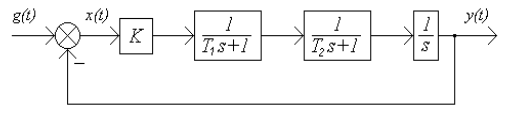
\includegraphics[scale = 0.8]{structureScheme}
        \caption{Структурная схема линейной системы третьего порядка}
    \end{figure}
    \clearpage
    \section{Нахождение границы устойчивости методом математического моделирования}
    При постоянных коэффициетах $T_1$ и $T_2$, изменяя значение коэффициента $K$, получим разные графики переходных процессов, соответствующие разным уровням устойчивости системы. Схема моделирования системы представлена на рисунке 2.
    \begin{figure}[h!]
        \centering
        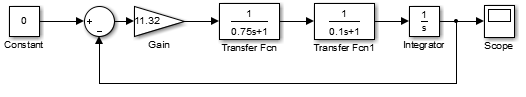
\includegraphics[scale = 1]{modelScheme.png}
        \caption{Схема моделирования заданной системы}
    \end{figure}
    
    На рисунке 3 представлены результаты моделирования, на которых полученны устойчивое положение системы, не устойчивое и 2 состояния на границе устойчивости: на нейстральной и колебательной.
    \begin{figure}[ht!]
        \begin{subfigure}[b]{0.49\textwidth}
            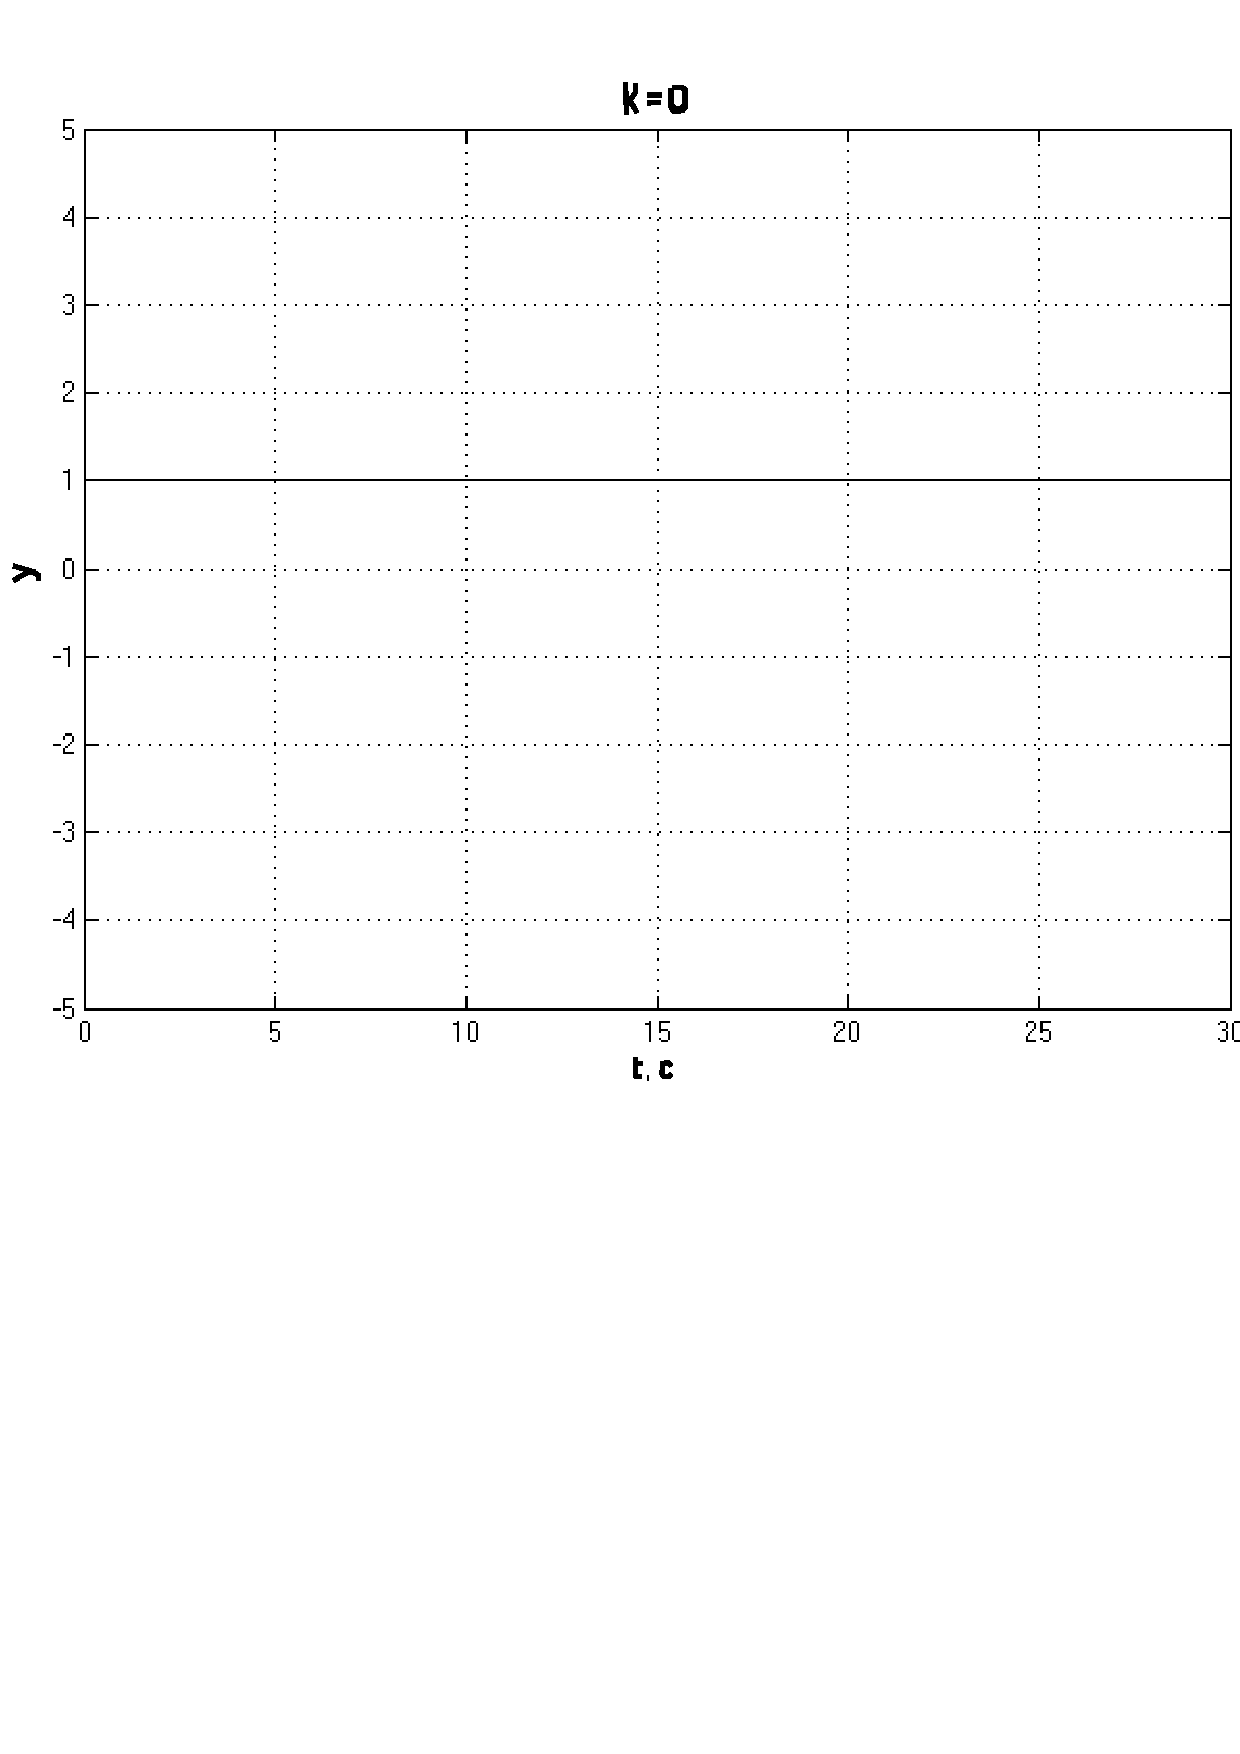
\includegraphics[width = \textwidth]{neutralStabilityLimit}
            \centering
            \caption{Нейстральная граница устойчивости}
        \end{subfigure}
        \hfill
        \begin{subfigure}[b]{0.49\textwidth}
            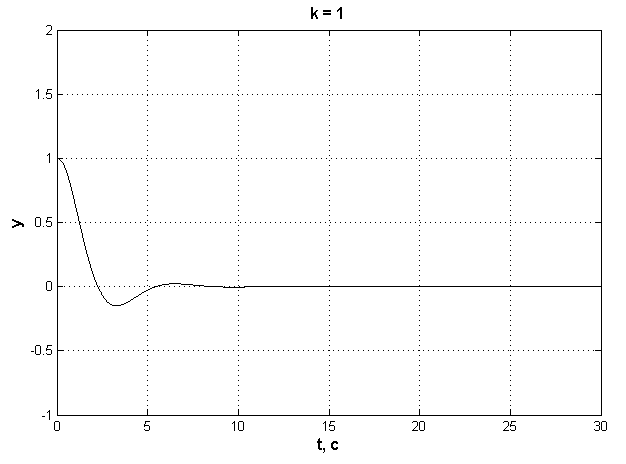
\includegraphics[width = \textwidth]{stable}
            \centering
            \caption{Устойчивое состояние}
        \end{subfigure}
        
        \begin{subfigure}[b]{0.49\textwidth}
            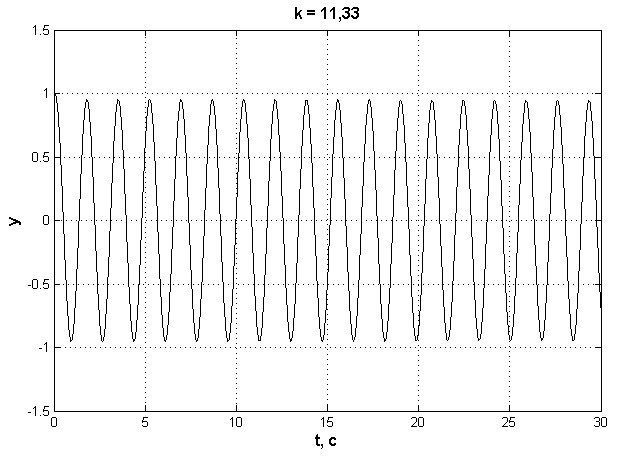
\includegraphics[width = \textwidth]{oscillatoryStabilityLimit}
            \centering
            \caption{Колебательная граница устойчивости}
        \end{subfigure}
        \hfill
        \begin{subfigure}[b]{0.49\textwidth}
            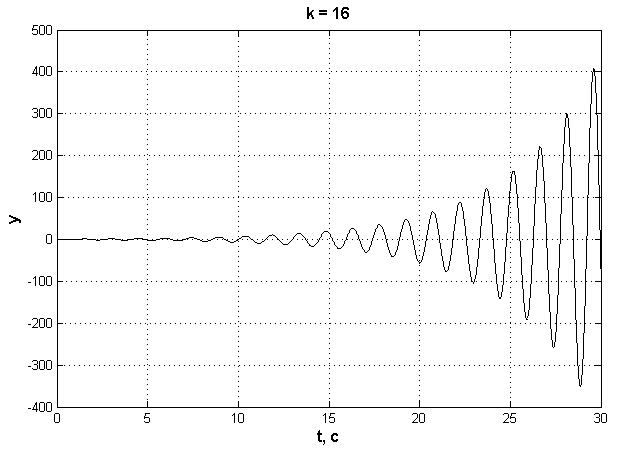
\includegraphics[width = \textwidth]{unstable}
            \centering
            \caption{Неустойчивое состояние}
        \end{subfigure}
        \caption{Переходные процессы системы при разных значениях коэффициента k}
    \end{figure}
    \clearpage
    \section{Теоретический расчёт параметров устойчивости системы}
    Рассчитаем передаточную функцию заскнутой системы
    $$W(s) = \frac{\Phi(s)}{1 + \Phi(s)}, \eqno (1)$$ где $\Phi(s)$ - передаточная функция разомкнутой системы.
    $$\Phi(s) = K\cdot\frac{1}{T_1s + 1}\cdot\frac{1}{T_2s + 1}\cdot\frac{1}{s} = \frac{K}{T_1T_2s^3 + (T_1 + T_2)s^2 +s}, \eqno (2)$$
    $$W(s) = \frac{(T_1T_2s^3 + (T_1 + T_2)s^2 +s)\cdot\displaystyle{\frac{K}{T_1T_2s^3 + (T_1 + T_2)s^2 +s}}}{T_1T_2s^3 + (T_1 + T_2)s^2 +s + K} = \frac{K}{T_1T_2s^3 + (T_1 + T_2)s^2 +s + K}. \eqno (3)$$
    
    На основании характеристического уравнения, построенного по передаточной функции замкнутой системы, составим матрицу Гурвица
    \[
    \begin{pmatrix}
        $$T_1 + T_2$$ & $$K$$ & 0\\
        $$T_1T_2$$ & 1 & 0\\
        0 & $$T_1 + T_2$$ & $$K$$
    \end{pmatrix}
    \]
    тогда главные миноры матрицы Гурвица равны
    $$D_1 = T_1 + T_2, \eqno (4)$$
    $$D_2 = 
    \begin{vmatrix}
        T_1 + T_2 & K\\
        T_1T_2 & 1
    \end{vmatrix}
    = T_1 + T_2 - T_1T_2K, \eqno (5)$$
    $$D_3 = D_2\cdot K = (T_1 + T_2)K - T_1T_2K^2. \eqno (6)$$
    
    По критерию Гурвица для устойчивости системы необходимо, чтобы главные миноры матрицы были положительны. Если минор $n - 1$ порядка равен 0, то система будет находится на колебательной границе устойчивости. Отсюда получаем уравнения коэффициентов для колебательной границы устойчивости
    \begin{equation*}
        \begin{cases}
            $$T_1 + T_2 > 0$$\\
            $$K = \displaystyle{\frac{T_1 + T_2}{T_1T_2}}$$
        \end{cases}
        \eqno (7)
    \end{equation*}
    
    Так как по нашему условию $T_1$ и $T_2$ больше 0, то единственным условием для того, чтобы система находилась на колебательной границе устойчивости, является
    $$K = \displaystyle{\frac{T_1 + T_2}{T_1T_2}}. \eqno (8)$$
    
    Используя полученное выражение, найдём $K$ для $T_1 = 0,75$ и $T_2$ изменяющемся от 0,1 с до 5 с с шагом 0,5 с. Полученны значения K запишем в таблицу 1.
    \begin{table}[h!]
        \centering
        \caption{Значения К для колебательной границы устойчивости системы}
        \begin{tabular}{|c|c|c|c|c|c|c|c|c|c|c|c|}
            \hline
            $T_2$ & 0,1 & 0,5 & 1 & 1,5 & 2 & 2,5 & 3 & 3,5 & 4 & 4,5 & 5 \\
            \hline
            $K$ & 11,33 & 3,33 & 2,33 & 2 & 1,83 & 1,73 & 1,66 & 1,62 & 1,58 & 1,56 & 1,53 \\
            \hline
        \end{tabular}
    \end{table}
    \newpage
    По полученным значениям построим график зависимости $K$ от $T_2$:
    \begin{figure}[ht!]
        \centering
        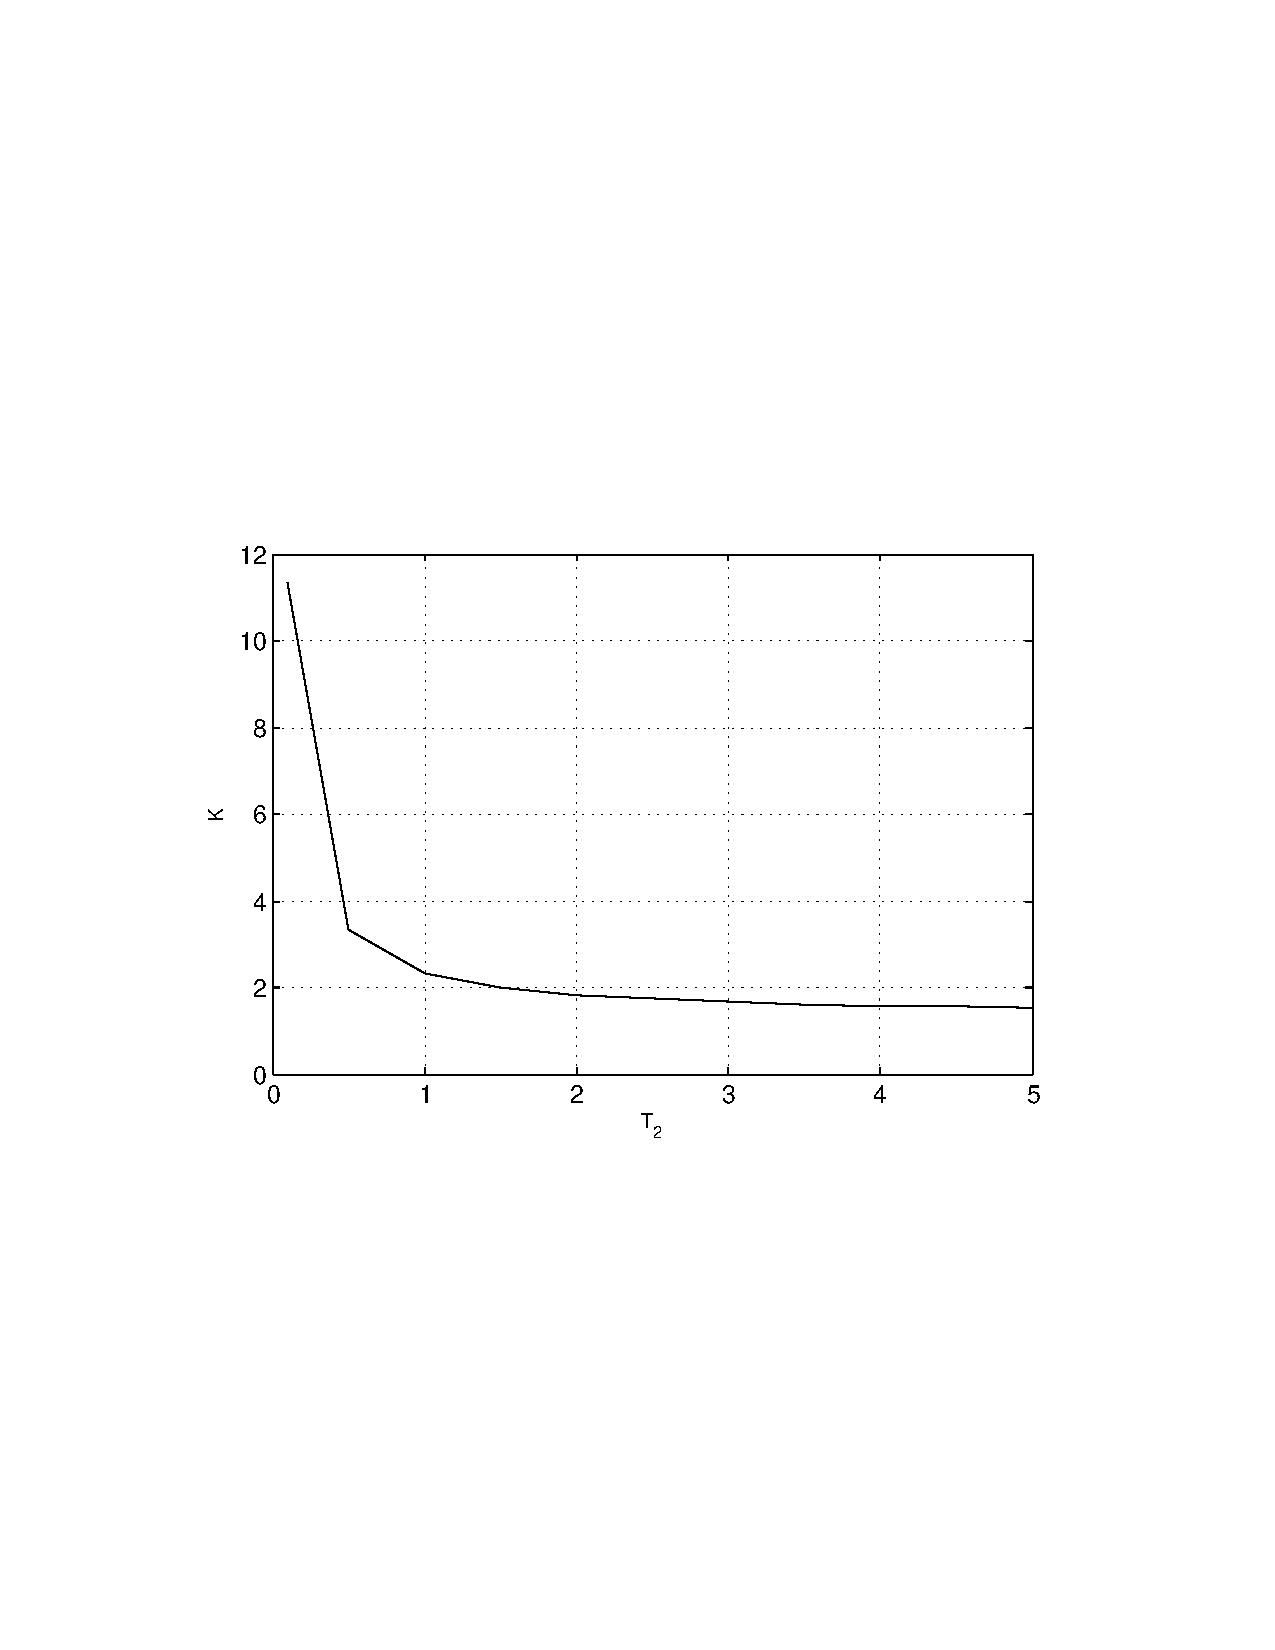
\includegraphics[width = \textwidth]{KT2graph}
        \caption{Граница устойчивости на плоскости двух параметров $K$ и $T_2$}
    \end{figure}
    \clearpage
    \section*{Вывод}
    В ходе работы был исследован способ управления устойчивастью системы, изменяя её параметры. Из трёх данных параметров $K, T_1$ и $T_2$ изменялись только $K$ и $T_2$. Аналитически и по средствам математического моделирования были рассчитаны значения, по которым был построен график границы устойчивости на плоскости двух параметров $K$ и $T_2$. Результаты, полученные обоими способами, совпадают.
\end{document}